\documentclass[12pt]{article}
\usepackage{enumerate, amsmath, fullpage, hyperref, amsfonts, titlesec, listings, graphicx, enumitem, longtable, tikz}
\usetikzlibrary{calc,trees,positioning,arrows,chains,shapes.geometric,
    decorations.pathreplacing,decorations.pathmorphing,shapes,
    matrix,shapes.symbols}
\renewcommand*\contentsname{Table of Contents}
\newlength\tindent
\setlength{\tindent}{\parindent}
\setlength{\parindent}{0pt}
\renewcommand{\indent}{\hspace*{\tindent}}
\lstset{
   breaklines=true,
   basicstyle=\scriptsize\rmfamily}
\tikzset{
>=stealth',
  chain/.style={
    rectangle, 
    rounded corners, 
    % fill=black!10,
    draw=black, very thick,
    text width=10em, 
    minimum height=3em, 
    text centered, 
    on chain},
  line/.style={draw, thick, <-},
  element/.style={
    tape,
    top color=white,
    bottom color=blue!50!black!60!,
    minimum width=8em,
    draw=blue!40!black!90, very thick,
    text width=10em, 
    minimum height=3.5em, 
    text centered, 
    on chain},
  every join/.style={->, thick,shorten >=1pt},
  decoration={brace},
  tuborg/.style={decorate},
  tubnode/.style={midway, right=2pt},
}
\begin{document}
\thispagestyle{empty}
\begin{center}
  {\bf\Large Train Control Demo 2 / Final Train Demo}\\
  {\bf\large CS452 - Spring 2014}\\
  Real-Time Programming\vspace{5cm}\\
  {\bf Team }\\
  Max Chen - mqchen\\
  mqchen@uwaterloo.ca\\[1\baselineskip]
  Ford Peprah - hkpeprah\\
  ford.peprah@uwaterloo.ca\vspace{5cm}\\
  Bill Cowan\\
  University of Waterloo\\
\end{center}
\newpage
% Program Description: how to operate it, full pathname
% Description fo structure of Kernel: algorithms, data structures, etc.
% Location fo source code + MD5
% Output produced by program and explanation of why it does
\thispagestyle{empty}
\tableofcontents
\newpage
\section{Program Description}
\subsection{Getting the Program}
To run the program, one must have read/write access to the source code, as well as the ability to make and run the program.  Before attempting to run the pogram ensure that the following three conditions are met:
\begin{itemize}
  \item You are currently logged in as one of \texttt{cs452}, \texttt{mqchen}, or \texttt{hkpeprah}.
  \item You have a directory in which to store the source code, \\ e.g. \texttt{\textasciitilde/cs452\_microkern\_mqchen\_hkpeprah}.
  \item You have a folder on the FTP server with your username, e.g. \texttt{/u/cs452/tftp/ARM/cs452}.
\end{itemize}
First, you must get a copy of the code.  To to this, log into one of the aforementioned accounts and change directories to the directory you created above (using \texttt{cd}), then run one of
\begin{center}
  \begin{verbatim}
    git clone file:////u8/hkpeprah/cs452-microkern -b final .
                           or
    git clone file:////u7/mqchen/cs452/cs452-microkern -b final .
  \end{verbatim}
\end{center}
\vspace{-0.5cm}You will now have a working instance of our TC2/Final source code in your current directory.  To make the application and upload it to the FTP server at the location listed above (\texttt{/u/cs452/tftp/ARM/YOUR\_USERNAME}), run \texttt{make upload}.  This will generate our source code that is functional on Track A, since distances are different on both tracks, you should run by specifying the track you want to use.  To do so, you can use any of the options listed below to customize your generated ELF file:
\begin{center}
  {\bf Make Options} - Can only specify one
  \begin{tabular}{|l|c|c|}
    \hline
    {\bf Option} & {\bf Description} \\\hline
    upload & Make and upload the generated file. \\\hline
    debug & Make and upload the generated file with debugging enabled. \\\hline
    test & Make for testing. \\\hline
  \end{tabular}
\end{center}
\begin{center}
  {\bf Make Flags} - Multiple can be specified
  \begin{tabular}{|l|c|c|}
    \hline
    {\bf Flag} & {\bf Description} \\\hline
    \texttt{TRACK=a} or \texttt{TRACK=b} & Makes for track A or track B depending on specified. \\\hline
    \texttt{SILENT} & Make with debugging off for tests. \\\hline
    \texttt{PROFILING} & Make for testing profiling. \\\hline
    \texttt{TEST=filename.c} & Make a test file using the specified file as the main. \\\hline
    \texttt{TARGET=filename} & Make the code and store it in the specified elf file. \\\hline
  \end{tabular}
\end{center}
\\[1\baselineskip]
\subsection{Running the Program}
To run the application, you need to load it into the RedBoot terminal.  Ensure you've followed the steps listed above in the ``Getting the Program'' settings to ensure you have the correct directories and account set up.  Navigate to the directory in which you cloned the source code and run \texttt{make upload}.  The uploaded code should now be located at (depending on the track you made for, defaults to 'a'):
\begin{center}
  \texttt{/u/cs452/tftp/ARM/YOUR\_USERNAME/kernel-a.elf} \\
  \texttt{/u/cs452/tftp/ARM/YOUR\_USERNAME/kernel-b.elf}
\end{center}
To run the application, go to the RedBoot terminal and run the command
\begin{center}
  \texttt{load -b 0x00218000 -h 10.15.167.4 ``ARM/YOUR\_USERNAME/kernel.elf''; go}
\end{center}
The application should now begin by running through the game tasks before reaching a prompt.  The generated files will be located in \texttt{DIR/build} where \texttt{DIR} is the directory you created in the earlier steps.  To access and download an existing version of the code, those can be found at \texttt{/u/cs452/tftp/ARM/mqchen/kernel.elf} and \texttt{/u/cs452/tftp/ARM/hkpeprah/kernel.elf}.
\\
\subsubsection{Command Prompt}
After the startup tasks have finished running, the user will reach a command prompt where they will be able to enter commands.  A list of available commands and the syntax can be found at run-time by entering either ``?'' or ``help'' followed by the ``RETURN'' key.  All commands must be followed by the ``RETURN'' key for the {\tt Shell} to interpret them.
\\[2\baselineskip]
\section{Task Structure}
\\[2\baselineskip]
\section{Train Control Demo 2}
\subsection{Train Calibration}
\subsubsection{Shortest Path Finding}
\subsubsection{Collision Avoidance}
\subsubsection{Reservation}
\subsubsection{Recovery}
\\[2\baselineskip]
\section{Final Demo - Transit System}
\subsection{Overview}
The final demo consists of modeling a transit system through the use of the kernel and code completed from Train Demo 1 and 2.  By using path finding, the trains are able to be routed to different stations (represented by sensors) to pick up passengers and bring them to their destination.  Each passenger has their own destination of one of the available stations; multiple passengers waiting at one station may each have a different destination.  Passengers and stations can be added at will or randomly as the user seems fit.  The transit system used in our project has been named ``Mr. Bone's Wild Ride''.
\\[1\baselineskip]
\subsection{Structure}
The following diagram outlines the structure of communication and routing works in the transit system.
\begin{center}
  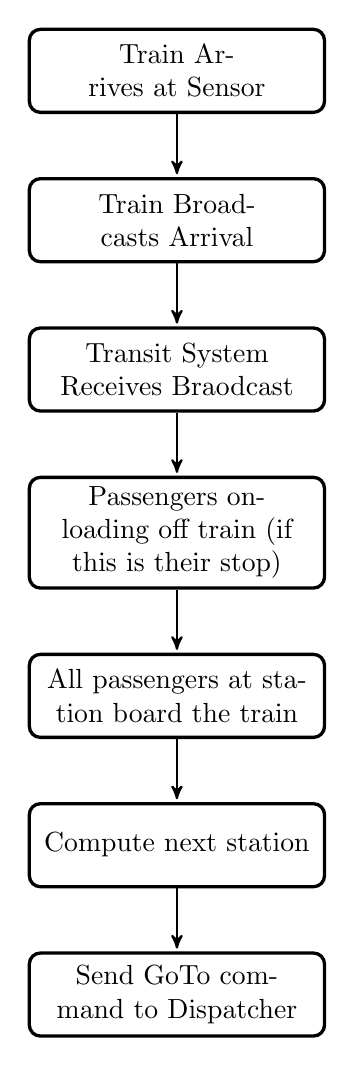
\begin{tikzpicture}[node distance=.8cm, start chain=going below,]
    \node[chain, join] (arrival) {Train Arrives at Sensor};
    \node[chain, join] (broadcast) {Train Broadcasts Arrival};
    \node[chain, join] (receive) {Transit System Receives Braodcast};
    \node[chain, join] (process) {Passengers on-loading off train (if this is their stop)};
    \node[chain, join] (process2) {All passengers at station board the train};
    \node[chain, join] (process3) {Compute next station};
    \node[chain, join] (send) {Send GoTo command to Dispatcher};
  \end{tikzpicture}
  \\[1\baselineskip]
\end{center}
\subsection{Station Allocation}
\\[1\baselineskip]
\subsection{Passenger System}
Each passenger in the system has their own destination.  Destinations are assigned ranedomly when a passenger is created at a station; a passenger may already be at the station of their choice, in which case they are simply done.  Each passenger has an associated weight which begins at $1$.  When determining which station a train should go to next, the system computes weights for each station as the sum of the weights of the passengers who want to go to that destination; the largest weighted station is the next station that train is routed to.  When a passenger is on a train and arrives at a station but does not get off (it is not their station), their weight increases by $1$.  This allows the system to account for situations where there would be only one passenger wanting to go to a particular station, and as a result, they would never get off because the other stations would be valued higher.  In addition, as a part of the passenger system, passengers also communicate to voice their opinions on the service to a channel that can be viewed by running the command ``intercom'' from within the \texttt{Shell}.  These get progressively billigerant the longer the passengers are on the train without reaching their destination.
\\[2\baselineskip]
\section{Known Errors}
\\[2\baselineskip]
\section{MD5}
\lstinputlisting{md5}
\end{document}
